\documentclass{article}
\usepackage[a4paper, total={170mm, 257mm}]{geometry}

\usepackage{graphicx}
\graphicspath{ {./images/} }

\usepackage{multicol}
\usepackage{hyperref}
\usepackage{tikz}
\usepackage{siunitx}

\title{SQA Summer Research Write Up}
\author{Cory Aitchison}
\date{Summer 2021}

\twocolumn
\begin{document}
\maketitle

\tikzset{every picture/.style={line width=0.75pt}} %set default line width to 0.75pt        

\section{Introduction}

Radio frequency (RF) reflectometry allows for high-bandwidth, low noise measurements of device resistances - including that of semiconductor hole spin qubits.

\emph{Outline}: Measurements of spin qubit devices require a complex experimental set-up, where multiple measurements techniques are used simultaneously (DC measurements, nanosecond voltage pulses, and continuous RF waves are often combined together). Therefore, experiments require specially designed electrical circuits. Prior to use with qubit devices the experimental circuits must be tested and characterised. For this project you will characterise the operation of our new high-frequency sample holders (aka Copenhagen boards). Part of the characterisation will include using a test device (an rf transistor) to simulate a quantum dot sample. The measurements will serve as the baseline for future measurements of hole spin qubit devices using the new sample board.

\emph{Outcomes}: Gain experience testing and working with state-of-the art experimental set-up. Become familiar with a measurement set-up used in several leading qubit research groups: The Copenhagen boards are currently being used by research groups at UNSW, and Microsoft qubit teams at USYD (D. Reilly), and at QDEV in Copenhagen (C. Marcus). Become familiar with the rf reflectometry measurement technique, which is widely used in spin qubit experiments. Learn the basic properties of semiconductor quantum dots. Understand the relationship between semiconductor quantum dots and current progress toward building a quantum computer.

\section{Results and Observations}
\subsection{Characterise Operation of an RF Switch}

\subsection{Basic DC Test of the Copenhagen Sample Board}

\subsection{Characterise the RLC response of the CPH Ciruit}


\begin{figure}[tp]
    \centering
    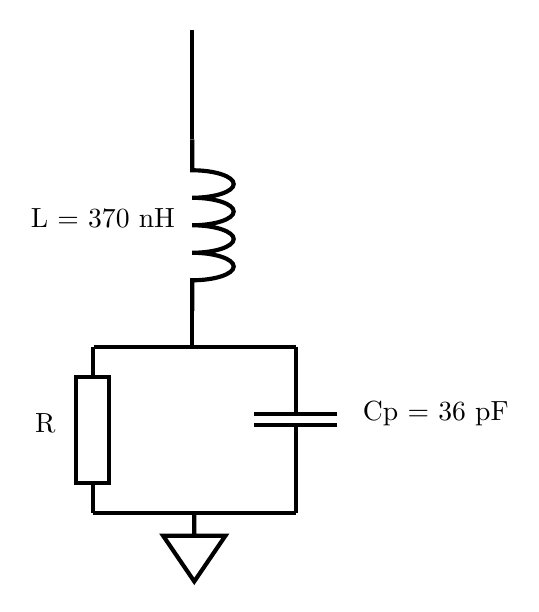
\begin{tikzpicture}[x=0.75pt,y=0.75pt,yscale=-1,xscale=1]
        %uncomment if require: \path (0,368); %set diagram left start at 0, and has height of 368

        %Straight Lines [id:da06782621221887086] 
        \draw [line width=1.5]    (290,27.2) -- (290,80) ;
        %Straight Lines [id:da7662482642077773] 
        \draw [line width=1.5]    (340,180) -- (242.5,180) ;
        %Shape: Resistor [id:dp8592626232820928] 
        \draw  [line width=1.5]  (250,194.4) -- (250,245.6) -- (234,245.6) -- (234,194.4) -- (250,194.4) -- cycle (242,180) -- (242,194.4) (242,245.6) -- (242,260) ;
        %Shape: Capacitor [id:dp2762209685239636] 
        \draw  [line width=1.5]  (340,190) -- (340,212.5) (360,217.5) -- (320,217.5) (360,212.5) -- (320,212.5) (340,217.5) -- (340,240) ;
        %Straight Lines [id:da6548911076200925] 
        \draw [line width=1.5]    (340,180) -- (340,190) ;
        %Straight Lines [id:da19597004940380347] 
        \draw [line width=1.5]    (340,240) -- (340,260) ;
        %Straight Lines [id:da8415802345776575] 
        \draw [line width=1.5]    (242,260) -- (340,260) ;
        %Shape: Ground [id:dp783868698411631] 
        \draw  [line width=1.5]  (276,271) -- (291,293) -- (306,271) -- (276,271) -- cycle (291,260) -- (291,271) ;
        %Shape: Inductor (Air Core) [id:dp42625766752857785] 
        \draw  [line width=1.5]  (290,80) -- (290,94.9) .. controls (301.04,94.9) and (310,97.87) .. (310,101.53) .. controls (310,105.18) and (301.04,108.15) .. (290,108.15) .. controls (301.04,108.15) and (310,111.12) .. (310,114.78) .. controls (310,118.43) and (301.04,121.4) .. (290,121.4) .. controls (301.04,121.4) and (310,124.37) .. (310,128.02) .. controls (310,131.68) and (301.04,134.65) .. (290,134.65) .. controls (301.04,134.65) and (310,137.62) .. (310,141.27) .. controls (310,144.93) and (301.04,147.9) .. (290,147.9) -- (290,162.8) ;
        %Straight Lines [id:da061679490108252466] 
        \draw [line width=1.5]    (290,162.8) -- (290,180) ;

        % Text Node
        \draw (211,112) node [anchor=north west][inner sep=0.75pt]   [align=left] {L = 370 nH};
        % Text Node
        \draw (371,205) node [anchor=north west][inner sep=0.75pt]   [align=left] {Cp = 36 pF};
        % Text Node
        \draw (213,211) node [anchor=north west][inner sep=0.75pt]   [align=left] {R};
    \end{tikzpicture}

    \caption{Circuit diagram of RLC circuit.}
    \label{fig:rlc_circuit}

\end{figure}

\begin{table}[htp]
    \centering
    \begin{tabular}{| c | c  | c | c |}
        \hline
        Inductor & $f_\mathrm{res}$ (\si{\mega\hertz}) & $L$ (\si{\nano\henry}) & $C_p$ (\si{\pico\farad}) \\[0.5ex]
        \hline \hline
        $L1$     & $164$                               & $1200$                 & $0.79$                   \\
        $L2$     & $192$                               & $820$                  & $0.84$                   \\
        $L3$     & $186$                               & $560$                  & $1.3$                    \\
        $L4$     & $50$                                & $390$                  & $26$                     \\ \hline
    \end{tabular}
    \caption{Measured resonant frequencies for each inductor on the Copenhagen board; inductances are given as per specifications; capacitances are calculated using the resonance formula $f_\mathrm{res} = 1/2\pi\sqrt{LC_p}$. As per Figure \ref{fig:transistor}, the inductors correspond to: $L1$ - not connected; $L2$ - not connected; $L3$ - gate; $L4$ - source.}
    \label{table:capacitances}
\end{table}

\subsection{Use RF Reflectometry to Characterise a Transistor}

\begin{figure}
    \caption{Transistor}
    \label{fig:transistor}
\end{figure}

\begin{figure}
    \caption{SMU Circuit}
    \label{fig:smu_circuit}
\end{figure}

Transistor is set up as per Figure \ref{fig:transistor}, with the SMU connected as per Figure \ref{fig:smu_circuit}

We see currents\dots

And resistances\dots

\subsection{Optimise the Reflectometry Circuit for Operation of the Transistor}

Take Equation \ref{eq:zt}.

\begin{figure}[tp]
    \centering
    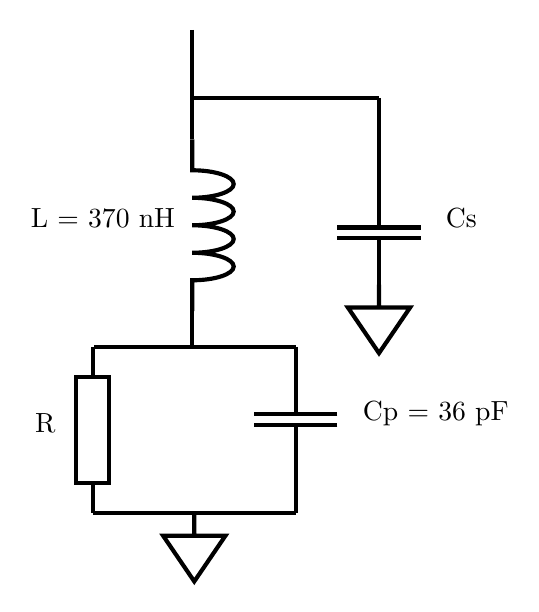
\begin{tikzpicture}[x=0.75pt,y=0.75pt,yscale=-1,xscale=1]
        %uncomment if require: \path (0,368); %set diagram left start at 0, and has height of 368

        %Straight Lines [id:da06782621221887086] 
        \draw [line width=1.5]    (290,27.2) -- (290,80) ;
        %Straight Lines [id:da05438248126058465] 
        \draw [line width=1.5]    (380,60) -- (290,60) ;
        %Straight Lines [id:da158345526126636] 
        \draw [line width=1.5]    (380,60) -- (380,100) ;
        %Shape: Capacitor [id:dp8567246814632112] 
        \draw  [line width=1.5]  (380,100) -- (380,122.5) (400,127.5) -- (360,127.5) (400,122.5) -- (360,122.5) (380,127.5) -- (380,150) ;
        %Straight Lines [id:da7662482642077773] 
        \draw [line width=1.5]    (340,180) -- (242.5,180) ;
        %Shape: Resistor [id:dp8592626232820928] 
        \draw  [line width=1.5]  (250,194.4) -- (250,245.6) -- (234,245.6) -- (234,194.4) -- (250,194.4) -- cycle (242,180) -- (242,194.4) (242,245.6) -- (242,260) ;
        %Shape: Capacitor [id:dp2762209685239636] 
        \draw  [line width=1.5]  (340,190) -- (340,212.5) (360,217.5) -- (320,217.5) (360,212.5) -- (320,212.5) (340,217.5) -- (340,240) ;
        %Straight Lines [id:da6548911076200925] 
        \draw [line width=1.5]    (340,180) -- (340,190) ;
        %Straight Lines [id:da19597004940380347] 
        \draw [line width=1.5]    (340,240) -- (340,260) ;
        %Straight Lines [id:da8415802345776575] 
        \draw [line width=1.5]    (242,260) -- (340,260) ;
        %Shape: Ground [id:dp783868698411631] 
        \draw  [line width=1.5]  (276,271) -- (291,293) -- (306,271) -- (276,271) -- cycle (291,260) -- (291,271) ;
        %Shape: Ground [id:dp21245550286994108] 
        \draw  [line width=1.5]  (365,161) -- (380,183) -- (395,161) -- (365,161) -- cycle (380,150) -- (380,161) ;
        %Shape: Inductor (Air Core) [id:dp42625766752857785] 
        \draw  [line width=1.5]  (290,80) -- (290,94.9) .. controls (301.04,94.9) and (310,97.87) .. (310,101.53) .. controls (310,105.18) and (301.04,108.15) .. (290,108.15) .. controls (301.04,108.15) and (310,111.12) .. (310,114.78) .. controls (310,118.43) and (301.04,121.4) .. (290,121.4) .. controls (301.04,121.4) and (310,124.37) .. (310,128.02) .. controls (310,131.68) and (301.04,134.65) .. (290,134.65) .. controls (301.04,134.65) and (310,137.62) .. (310,141.27) .. controls (310,144.93) and (301.04,147.9) .. (290,147.9) -- (290,162.8) ;
        %Straight Lines [id:da061679490108252466] 
        \draw [line width=1.5]    (290,162.8) -- (290,180) ;

        % Text Node
        \draw (211,112) node [anchor=north west][inner sep=0.75pt]   [align=left] {L = 370 nH};
        % Text Node
        \draw (411,112) node [anchor=north west][inner sep=0.75pt]   [align=left] {Cs};
        % Text Node
        \draw (371,205) node [anchor=north west][inner sep=0.75pt]   [align=left] {Cp = 36 pF};
        % Text Node
        \draw (213,211) node [anchor=north west][inner sep=0.75pt]   [align=left] {R};

    \end{tikzpicture}
    \caption{Circuit diagram for optimised RF reflectometry circuit.}
    \label{fig:opt_circuit}
\end{figure}

\begin{equation}
    Z_t = \left[ \left(i\omega L + \frac1{\frac1R + i\omega C_p}\right)^{-1} + i\omega C_s \right]^{-1}
    \label{eq:zt}
\end{equation}

\begin{figure}[tp]
    \centering
    \includegraphics[scale=0.6]{S11_cs.png}
    \caption{S11}
    \label{fig:s11_cs}
\end{figure}

\section{Other accomplishments}

\begin{itemize}
    \item Updated AWG Pulse Studio for MATLAB v2 and implemented a parametric function option
    \item Updated AWG Pulse Studio documentation
    \item Updated VNA driver for MATLAB v2
    \item Created a driver for Keithley SM2401 source meter in MATLAB v2
    \item Dipped a sample (BBR) and performed a leak test of the gates at $4$ \si{\milli\kelvin}
\end{itemize}



\section{References}
\end{document}